\documentclass[aspectratio=169, table]{beamer}

%\usepackage[beamertheme=./praditatheme]{Pradita}
\usepackage[utf8]{inputenc}

\usetheme{Pradita}

\subtitle{MTI102-Information System \&\\Technology Architecture}

\title{Phase B:\\Business Architecture in TOGAF\\
     Architecture Development Method}
\date[Serial]{\scriptsize {PRU/SPMI/FR-BM-18/0222}}
\author[Pradita]{\small {\textbf{Alfa Yohannis}}}

\begin{document}

    \frame{\titlepage}

    \begin{frame}
        \frametitle{Goals}
        \begin{enumerate}
            \item Build a Target Business Architecture that describes how the company should operate to achieve business objectives, and respond to the strategic business drivers set out in the Architectural Vision, in a way that meets or answers \textit{Demand for Architectural Work} and \textit{things that be of concern to stakeholders}.

            \item Identify components of the Architecture Roadmap based on the gaps between the Current Architecture and the Target Business Architecture.
        \end{enumerate}
    \end{frame}

    \begin{frame}
        \frametitle{Input (1)}
        \begin{columns}
            \begin{column}{0.5\textwidth}
                \begin{center}
                    \begin{enumerate}

                        \item Business principles, business goals, and business drivers
                        \item Capability Assessment
                        \item Communication Plan
                        \item Organizational Models for Enterprise Architecture
                        \item Customized Architectural Framework
                        \item Approved Architectural Statement of Work

                    \end{enumerate}
                \end{center}
            \end{column}
            \begin{column}{0.5\textwidth}
                \begin{center}
                    \begin{enumerate}
                        \setcounter{enumi}{7}
                        \item Architectural Principles, including pre-existing business principles
                        \item Company Continuum
                        \item Architectural Repository
                        \item Architectural Vision, including:
                        \begin{itemize}
                            \item Problem
                            \item Purpose of Architectural Work Statement
                            \item Overview summary
                            \item Business scenario (optional)
                            \item Detailed high-level stakeholder requirements
                        \end{itemize}

                    \end{enumerate}
                \end{center}
            \end{column}
        \end{columns}
    \end{frame}

    \begin{frame}
        \frametitle{Input (2)}
        \begin{enumerate}
            \setcounter{enumi}{11}
            \item Draft Architectural Definition Document, including (if in scope):
            \begin{itemize}
                \item Basic Business Architecture (high level)
                \item Basic Data Architecture (high level)
                \item Basic Application Architecture (high level)
                \item Basic Technology Architecture (high level)
                \item Target Business Architecture (high level)
                \item Target Data Architecture (high level)
                \item Target Application Architecture (high level)
                \item Target Technology Architecture (high level)
            \end{itemize}
            \item Request for Architectural Work
        \end{enumerate}
    \end{frame}

    \begin{frame}
        \frametitle{Steps}
        \begin{enumerate}
            \item Select reference models, viewpoints of various actors, and tools
            \item Developing a Description of the Current Business Architecture
            \item Develop Target Business Architecture Description
            \item Conduct a Gap Analysis
            \item Defines the components of the roadmap
        \end{enumerate}


    \end{frame}

    \begin{frame}
        \frametitle{Steps(2)}
        \begin{enumerate}
            \setcounter{enumi}{5}
            \item Create solutions to impacts/side effects across the Architectural Landscape
            \item Conduct a formal stakeholder review of the proposed architecture.
            \item Complete the Business Architecture
            \item Create an Architecture Definition Document
        \end{enumerate}


    \end{frame}


    \begin{frame}
        \frametitle{Output}
        \begin{enumerate}
            \item Architectural Statement of Work, updated as necessary
            \item Validated business principles, business objectives, and business drivers
            \item Updated Principles of Business Architecture
            \item Draft Architectural Definition Document, including updated content
            \item Draft Architectural Requirements Specification, including updated content
            \item Business Architecture Components of the Architecture Roadmap
        \end{enumerate}
    \end{frame}

    \begin{frame}
        \frametitle{Using the Architecture Repository}
        \framesubtitle{\hspace{1cm}}
        Architecture teams need to consider relevant Business Architecture resources available from the Architecture Repository, especially:
        \begin{enumerate}
            \item general standards that apply
            \item Generic business models relevant to the organization's industry sector (retail and healthcare industries)
            \item Business models relevant to the business domain (medical device retail)
            \item Company-specific building blocks (process components, business rules, job descriptions, etc.)

        \end{enumerate}
    \end{frame}


    \begin{frame}
        \frametitle{Identifying Catalogs, Matrix, and Diagrams}
        \framesubtitle{\hspace{1cm}}
        \begin{enumerate}
            \item Catalogs collect an inventory of a business's core assets.
            \item The matrix shows the relationships between model entities.
            \item Diagrams depict Business Architecture information from various perspectives (views).
        \end{enumerate}
    \end{frame}

{
    \setbeamertemplate{navigation symbols}{}
    \setbeamertemplate{footline}{}
    \begin{frame}
        \centering
        \frametitle{Catalog, Matrix, and Diagram}
        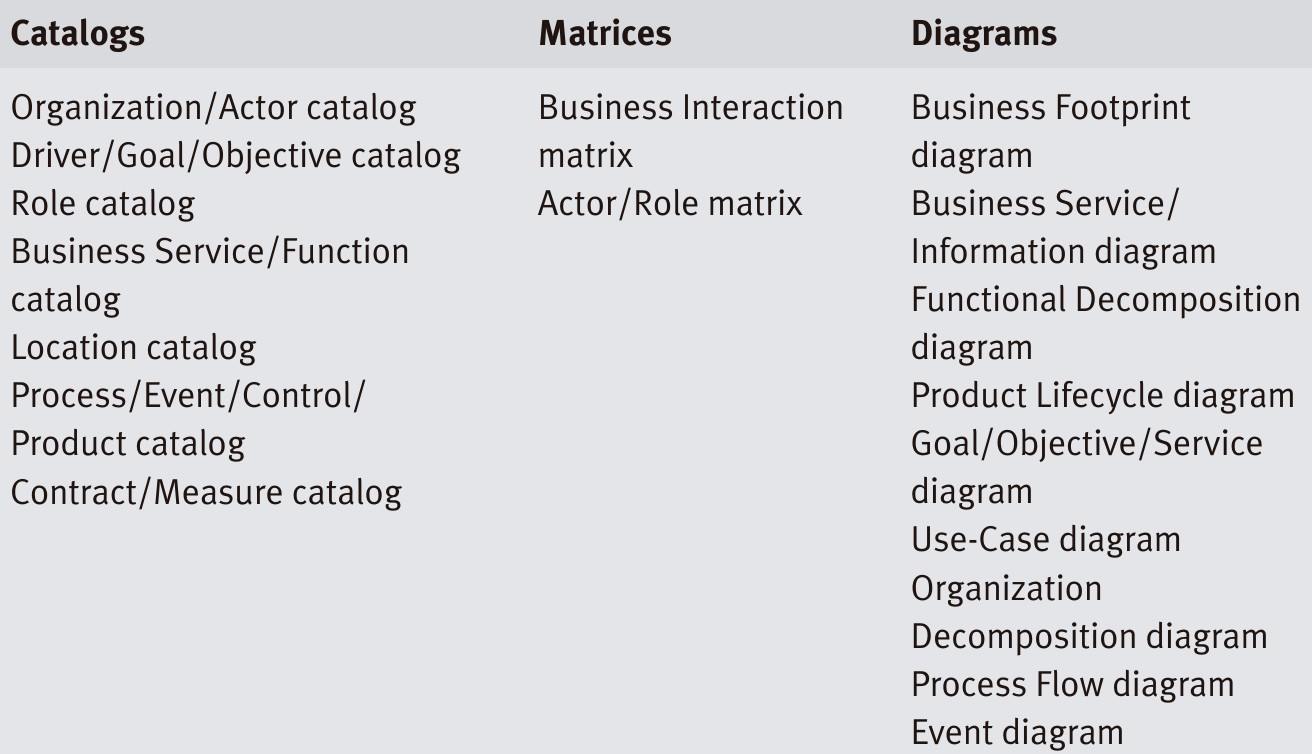
\includegraphics[width=.6\textwidth]{../figures/catalogs_matrices_diagrams.png}
    \end{frame}
}

\begin{frame}
    \frametitle{Contents of Architecture Definition Document}
     \framesubtitle{\hspace{1cm}}
    \begin{columns}
        \begin{column}{0.5\textwidth}
            \begin{center}
                \begin{enumerate}
                    \item Scope
                    \item Goals, objectives, and constraints
                    \item Architectural principles
                    \item Basic architecture
                    \item Architectural model (for each state to be modeled); such as models for Business Architecture, Data Architecture, Application Architecture, and Technology Architecture

                \end{enumerate}
            \end{center}
        \end{column}
        \begin{column}{0.5\textwidth}
            \begin{center}
                \begin{enumerate}
                    \setcounter{enumi}{5}
                    \item Rationale and justification for architectural approaches
                    \item Mappings to Architectural Repositories, including mappings to Architectural Landscapes, reference models, standards, as well as reuse assessments
                    \item Gap analysis
                    \item Impact assessment
                    \item Transitional Architecture
                \end{enumerate}
            \end{center}
        \end{column}
    \end{columns}
\end{frame}

\begin{frame}
    \frametitle{Contents of Business Architecture Components}
     \framesubtitle{\hspace{1cm}}
    \begin{enumerate}
        \item Business Architecture Baseline, if applicable; this is a description of the existing Business Architecture.
         \item Target Business Architecture.
         \item Both are best if they can cover:
        \begin{itemize}
        	\item \textbf{Views}that align with selected views to address key stakeholder concerns.
        	\item \textbf{Organizational structure} that identifies business locations and links them to organizational units.
        	\item \textbf{Business goals and objectives} for the company and each organizational unit.
        	\item \textbf{Business functions} are identified using detailed, recursive steps involving sequential decomposition of major functional areas into sub-functions.
        	\item \textbf{Business services} provided by the company and each company unit to its customers, both internal and external.
        \end{itemize}
    \end{enumerate}
\end{frame}


\begin{frame}
    \frametitle{Contents of Business Architecture Components (2)}
     \framesubtitle{\hspace{1cm}}
    \begin{itemize}
        \item \textbf{Business processes}, including measures and results produced.
        \item \textbf{Business role}, including development and modification of skill requirements.
        \item \textbf{Business data model}.
        \item \textbf{Organizational and functional correlation} that connects business functions with organizational units in the form of a matrix report.
    \end{itemize}
\end{frame}



\begin{frame}
    \frametitle{Fill in the Architectural Requirements Specification}
    \framesubtitle{\hspace{1cm}}
    \begin{columns}
        \begin{column}{0.5\textwidth}
            \begin{center}
                \begin{enumerate}
                    \item Measure of success
                    \item Architectural requirements
                    \item Business services contracts
                    \item Application service contract
                    \item Implementation guide
                    \item Implementation specifications

                \end{enumerate}
            \end{center}
        \end{column}
        \begin{column}{0.5\textwidth}
            \begin{center}
                \begin{enumerate}
                    \setcounter{enumi}{6}
                    \item Standard implementation
                    \item Interoperability requirements
                    \item IT service management requirements
                    \item Constraints
                    \item Assumptions
                \end{enumerate}
            \end{center}
        \end{column}
    \end{columns}
\end{frame}

\begin{frame}
    \frametitle{Business Architecture Requirements}
     \framesubtitle{\hspace{1cm}}
    \begin{enumerate}
        \item Gap Analysis Results
        \item Updated business requirements, identified using Business Scenario techniques
    \end{enumerate}
\end{frame}

\begin{frame}
    \frametitle{Business Architecture Requirements (2)}
     \framesubtitle{\hspace{1cm}}
    \begin{enumerate}
        \setcounter{enumi}{2}
        \item Technical requirements: An initial set of technical requirements should be generated as the output of Phase B: Business Architecture. This serves as the impetus for future Technology Architecture work, and should identify, categorize, and prioritize implications for work in the remaining architectural domains; for example, by using a dependency/priority matrix (e.g., guiding the trade-off between transaction processing speed and security) and a list of expected custom models is generated.

    \end{enumerate}
\end{frame}


\begin{frame}
    \frametitle{Summary}
    % \framesubtitle{\hspace{1cm}}
    \begin{enumerate}
        \item The Business Architecture phase allows us to define and validate the business architecture required to support the business strategy.
        \item This phase is important to ensure that the business architecture is aligned with stakeholder needs.
    \end{enumerate}
\end{frame}

{
	\setbeamertemplate{navigation symbols}{}
	\setbeamertemplate{footline}{}
	\begin{frame}
		\centering
		\begin{columns}[t]
			\begin{column}{.5\textwidth}
					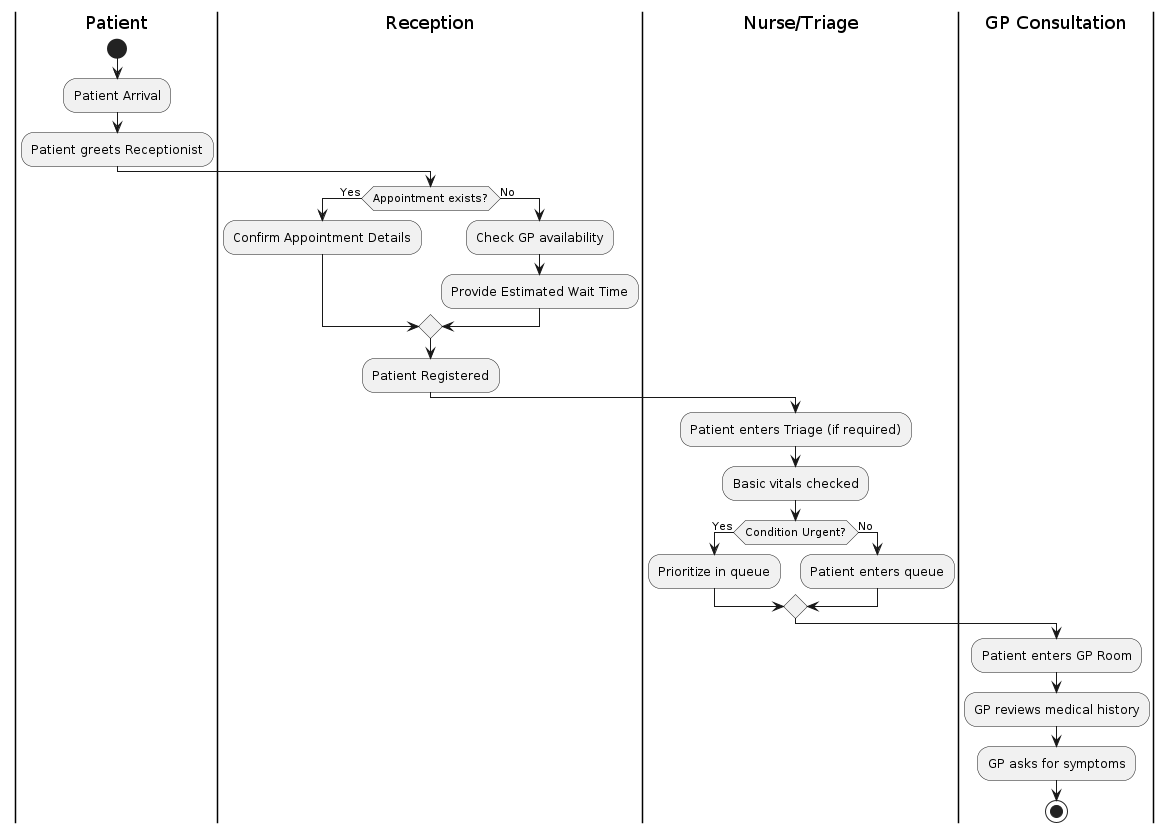
\includegraphics[width=\textwidth]{../figures/workflow_offline.png}
			\end{column}
			\begin{column}{.5\textwidth}
	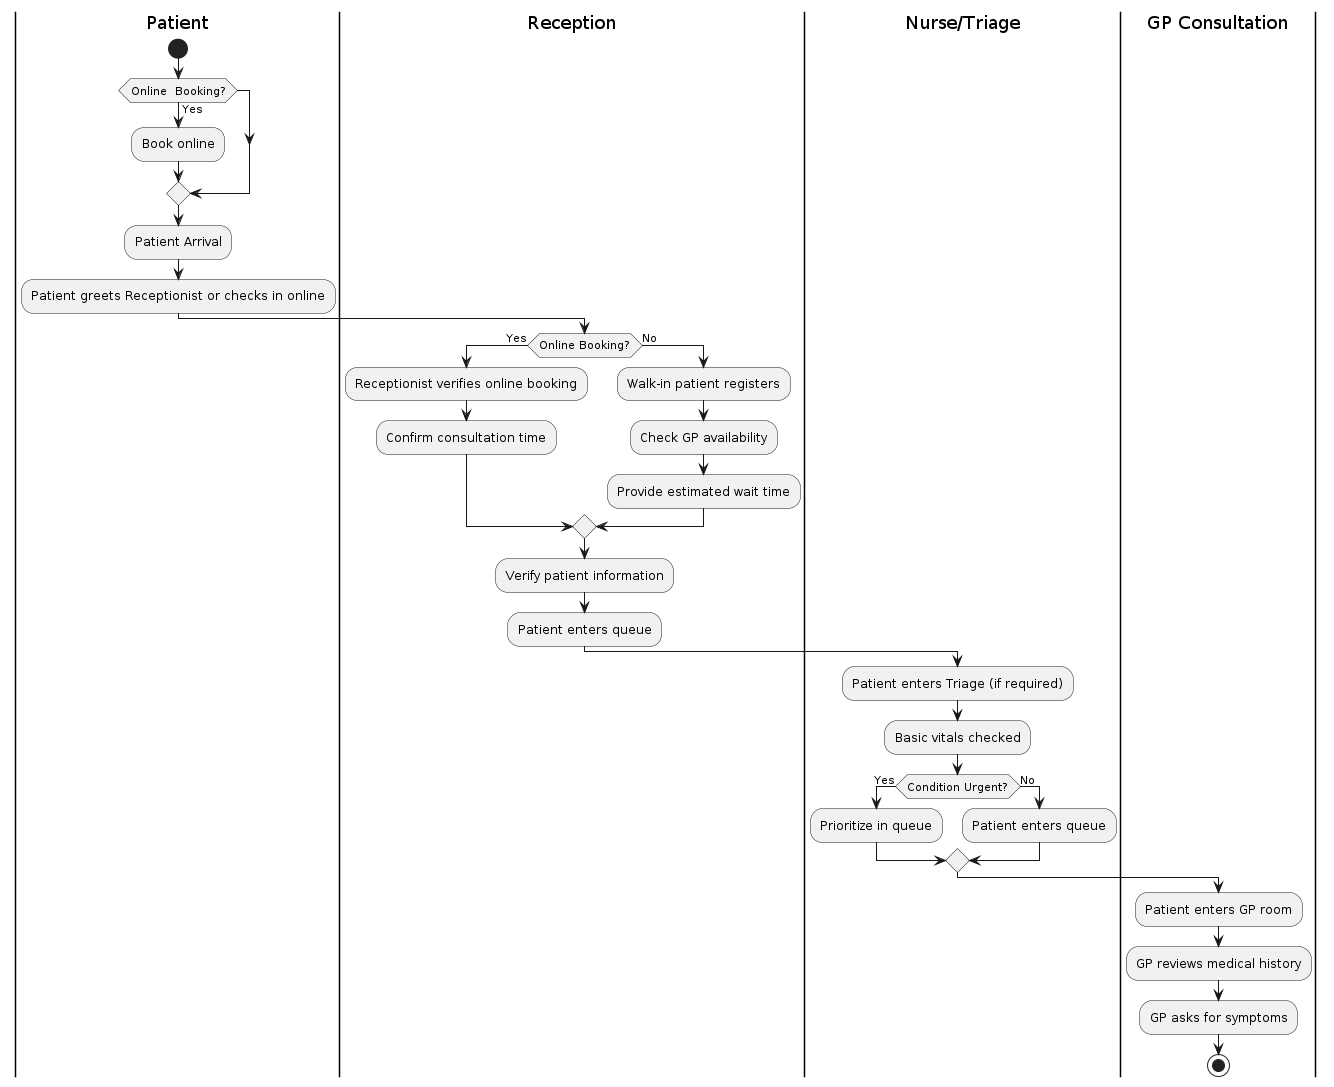
\includegraphics[width=\textwidth]{../figures/workflow_online.png}
			\end{column}
		\end{columns}
	\end{frame}
}

\end{document}
